\documentclass[preprint,review,12pt]{elsarticle}

\usepackage{amssymb}
\usepackage{graphicx}
\usepackage{multirow}
\usepackage{tabularx}
\usepackage{booktabs}
\usepackage[noend]{algpseudocode}
\usepackage{subfig}
\usepackage[table,xcdraw]{xcolor}
\usepackage{amsthm}
\usepackage{color}
\usepackage{soul}
\usepackage{ulem}
\usepackage{amsmath}
\usepackage{float}

\newcommand{\hlr}[2][red]{
  {\sethlcolor{#1} \hl{#2}}
}

\newcommand{\hly}[2][yellow]{
  {\sethlcolor{#1} \hl{#2}}
}
\newcommand{\hlg}[2][green]{
  {\sethlcolor{#1} \hl{#2}}
}
\newcommand{\hlp}[2][pink]{
  {\sethlcolor{#1} \hl{#2}}
}

\usepackage{lineno,hyperref}
\modulolinenumbers[5]

\journal{Journal of \LaTeX\ Templates}

\bibliographystyle{elsarticle-num}

\begin{document}

\begin{frontmatter}

\title{Joint Service Chain Deployment and Manager Placement in NFV}

\author[aut]{Parham Alvani
%طبق قوانین دانشگاه استاد باید باشد
%\corref{correspondingauthor}
}
\ead{parham.alvani@aut.ac.ir}
\author[aut]{Bahador Bakhshi
\corref{correspondingauthor}}
\ead{bbakhshi@aut.ac.ir}

\cortext[correspondingauthor]{Corresponding author.}

\address[aut]{Amirkabir University of Technology, Tehran, Iran}

\begin{abstract}
\hly{%
a) Motivation \\
b) Introduce the problem \\
c) Why is there a research gap \\
d) What have we done \\
e) What are the results \\
}

In the old times, Network providers use physical network functions to create their service chains, but a change in this manner is difficult and may cause many service disruptionn.
SFC and NFV is the solution to this difficulty. By using SFC and NFV, providers can provision chains dynamically and then change them in runtime.
One of the main requirements is management and monitoring for the chains.
In this research, we consider the chain acceptance problem subject to management resources. In the first step, we formulate
problem with ILP and then implement it in CPLEX framework. As we know, ILP problems are NP-Hard, so we need a Polynomial-Time solution to the problem.
In this research, we develop a heuristic algorithm and compare its result with the optimal solution. In the end, the heuristic solution produces near-optimal results in the polynomial time.
\end{abstract}

\begin{keyword}
\end{keyword}

\end{frontmatter}

\section{Introduction}
In NFV ecosystem, each chain must be monitored and managed by a VNFM. Similar to other virtual functions, VNFMs need computing and network resources and  can manage a limited number of chains.
Our work considers Service Chain Placement Problem and Manager Placement Problem jointly and wants to place chains and their corresponding VNFM at the same time.
We believe this work hasn't been done in the literature before.
By considering the joint problem, you may not accept a chain that you don't have any management resource for it,
or you can get many chains that have little management resource requirement.
These considerations create a better solution with more profit to datacenter from provisioning the set of chains,
and the results in \ref{sec:joint-vs-disjoint} approves it.


\hly{%
a) A general introduction of the context \\
b) More specific context of problem and its importance \\
c) A very brief review of literature and introduce the research gap \\
d) What is the problem \\
e) What are the contributions \\
f) The structure of the paper \\
}


\section{Related Work}
In this section, we review the works that have been done on service chain deployment and resource assignment in NFV, and mainly we focus on the works that consider management requirements of chains.

In NFV, resource assignment is composed of
allocating computing and memory resources for virtual machines to run the chains' virtual network functions and assigning network resources to the chains' virtual links. Various objective functions, e.g., minimizing cost, maximizing profit and minimizing power consumption can be aimed in the resource management problem where a wide range of additional, e.g., end-to-end delay, fault tolerance as well as management requirements need to be satisfied.

\subsection{Resource Allocation in NFV}
The VNF placement problem has received substantial attention in the literature \cite{GilHerrera2016}.
We will concentrate on network function chain placement which dynamically steers
traffic through an ordered list of Service Functions from 3 categories that are discussed in \cite{Laghrissi2019}.
Objectives like energy consumption minization, cost optimization, Quality of Service (QoS), resource usage, reliablity,
and load balancing.

\subsection{Management Resources in NFV}
As already mentioned, this work considers management resources. To best of our knowledge, work \cite{AbuLebdeh2017}, its next work \cite{AbuLebdeh20172}, and \cite{Chiang2019} are the only ones that consider VNFM and other management resources in SFC deployment.

In \cite{AbuLebdeh2017}, the authors studied the problem of VNFM placement in a distributed NFV infrastructure under the assumption that chains have already been deployed and consequently, the location of VNFs are known.
The objective function of the VNFM placement problem is to minimize the operational costs which is:
\begin{itemize}
    \item Life cycle Management Cost
    \item Compute Resources Cost
    \item Migration Cost
    \item Reassignment Cost
\end{itemize}
Delay constraint on management links is also considered.
The authors used tabu search algorithm because of its superior results to other techniques in FLP, for finding a polynomial solution. They start from a feasible placement and each step they improve VNFM placement by doing one of these moves:
\begin{itemize}
    \item Reassignment
    \item Relocation
    \item Bulk
    \item Deactivation
\end{itemize}
While this is the first work that investigated the management resource assignment in NFV, it does not the joint SFC deployment and VNFM placement.

In \cite{AbuLebdeh20172} authors solve VNFO placement problem that is far from our current work that doesn't consider VNFO.
Authors consider the same system as \cite{AbuLebdeh2017} but here they want to place VNFO and VNFM jointly, trying to minimize operational cost as defined by \cite{AbuLebdeh2017}.
They propose a two step placement algorithm that first place VNFOs and then place VNFMs. Each of these steps use Tabu-Search method.

In \cite{Chiang2019} authors consider autonomy for VNFMs that selects their managed VNFs dynamically and use game theory to achieve a distributed solution to the VNFM Placement Problem as desribed in \cite{AbuLebdeh2017}.
Authors consider the same system model from \cite{AbuLebdeh2017} and try minimize operational cost consists of bandwidth cost and compute cost.
In our work relation between VNFMs and VNFs are static and VNFM cannot change these relation by their own.

To conclude, the problem of joint SFC deployment and VNFMs placement has not yet been consider. In the rest of this paper, we formulate the problem and propose solution for it.

\subsection{Current Work}

Our work considers the above problems jointly and wants to place chains and their corresponding VNFM at the same time.
We believe this work hasn't been done in the literature before.
By considering the joint problem, you may not accept a chain that you don't have any management resource for it,
or you can get many chains that have little management resource requirement.
These considerations create a better solution with more profit to datacenter from provisioning the set of chains,
and the results in \ref{sec:joint-vs-disjoint} approves it.
The closest work to current research is \cite{AbuLebdeh2017} but it assumes that the VNFs' placement is known and solves only the VNF manager placement problem. Current research also considers more constraints that \cite{AbuLebdeh2017} on VNFM placements that we discuss deeply in the following sections and summarize them here:

\begin{itemize}
    \item Current research considers license cost for VNFM instances
    \item In current research each physical node has its specific list of nodes that can run its VNFM. This constraint provides a great flexibility for implementing management policies.
\end{itemize}

At the end current research and \cite{AbuLebdeh2017} have different objectives but we will try to compare their results and solutions.


\section{System Model and Problem Statement}
\hly{
a) Assumptions \\
b) System model \\
Table of notations \\
c) Problem statement \\
Define the problem in English using the notations and finally give an illustrative example to clarify the \\
problem
}

\section{Problem Formulation}
\hly{
a) Define variables and parameters \\
b) Define objective function \\
c) Define constraints \\
d) Put the objective function and constraints together and define the problem \\
e) State the complexity of the model (NP-Hardness) \\
}

\section{Proposed Solution}
\hly{
a) Use the top-down approach. At be beginning draw a big picture of the solution steps \\
b) Explain the details of the steps. Emphasize the idea behind the heuristic decisions \\
c) Put all them together as a pseudo code or flowchart \\
d) Analyze the complexity of the proposed solution \\
}

\section{Evaluation and Numerical Results}
\hly{
a) Simulation settings: Topologies and all other parameters used in simulation it is better to use a table \\
The algorithms which are simulated \\
Parameters used for evaluation \\
b) A subsection per parameter\\
Emphasize on achievements\\
}
\subsection{Joint vs Disjoint}\label{sec:joint-vs-disjoint}
Here we want to compare the joint and disjoint solutions.
For this comparison we use two different topology to have better insights and fair results.

\subsubsection{FatTree}
Here we will use FatTree topology with k equals to 6.
As you can see results confirm our hypothesis that joint solutions makes better revenues.

\begin{table}[H]
    \caption{Revenues from Joint and Disjoint Solutions on FatTree Topology with k equals to 6}
    \label{tbl:joint-vs-disjoin-fattree}
    \medskip
    \centering
    \begin{tabular}{lrrr}
        \toprule
        {} &    joint &  disjoint &  nchains \\
        \midrule
        0 &  45440.0 &   44980.0 &      100 \\
        1 &  36660.0 &   17090.0 &       80 \\
        2 &  27850.0 &   13340.0 &       60 \\
        3 &  18340.0 &   13440.0 &       40 \\
        4 &   9170.0 &    1880.0 &       20 \\
        \bottomrule
    \end{tabular}
\end{table}

\begin{figure}[H]
    \centering
    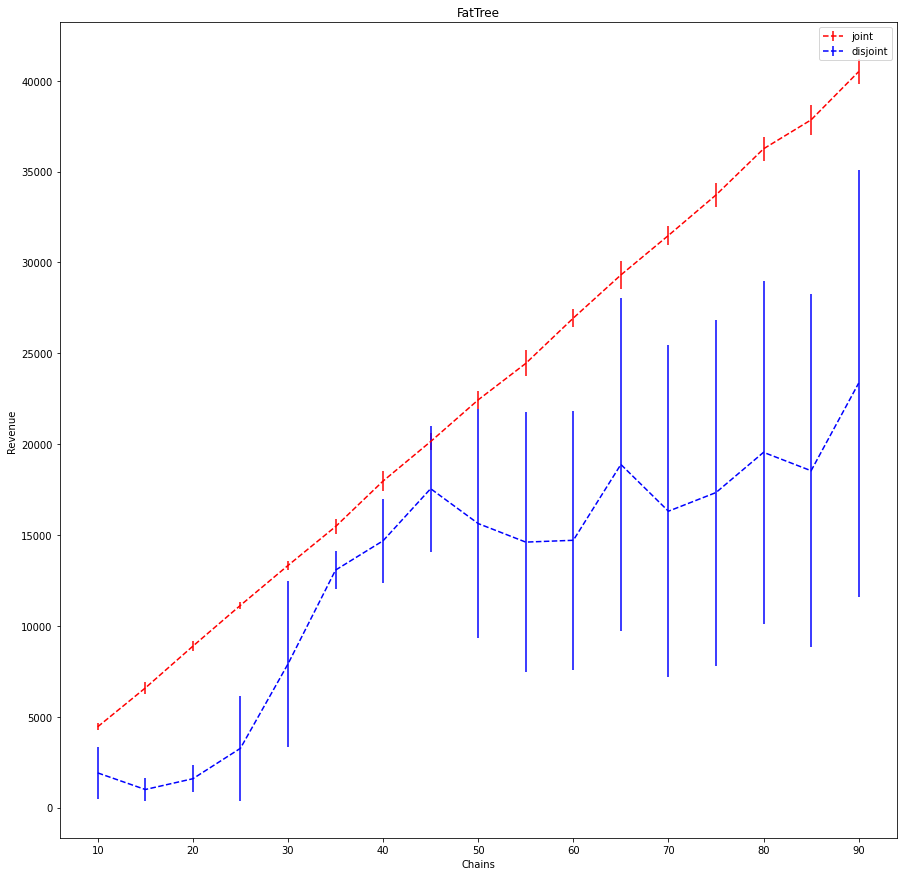
\includegraphics[height=350pt]{plots/joint-vs-disjoint-fattree.png}
    \caption{Revenues from Joint and Disjoint Solutions on FatTree Topology with k equals to 6}
    \label{fig:joint-vs-disjoint-fattree}
\end{figure}

\subsection{USNet}
Here we will use USNet topology with 3 to 4 nodes attached to each of its points.
As you can see the results show joint and disjoint solutions on this setup work equally because there is no specific
management requirement and topology can handle all chains.

\begin{table}[H]
    \caption{Revenues from Joint and Disjoint Solutions on USNet Topology}
    \label{tbl:joint-vs-disjoin-usnet}
    \medskip
    \centering
    \begin{tabular}{lrrr}
        \toprule
        {} &    joint &  disjoint &  nchains \\
        \midrule
        0 &  23000.0 &   23010.0 &       50 \\
        1 &  34180.0 &   34260.0 &       75 \\
        2 &  45430.0 &   45560.0 &      100 \\
        3 &  57180.0 &   57380.0 &      125 \\
        4 &  68750.0 &   69360.0 &      150 \\
        \bottomrule
    \end{tabular}
\end{table}

\begin{figure}[H]
    \centering
    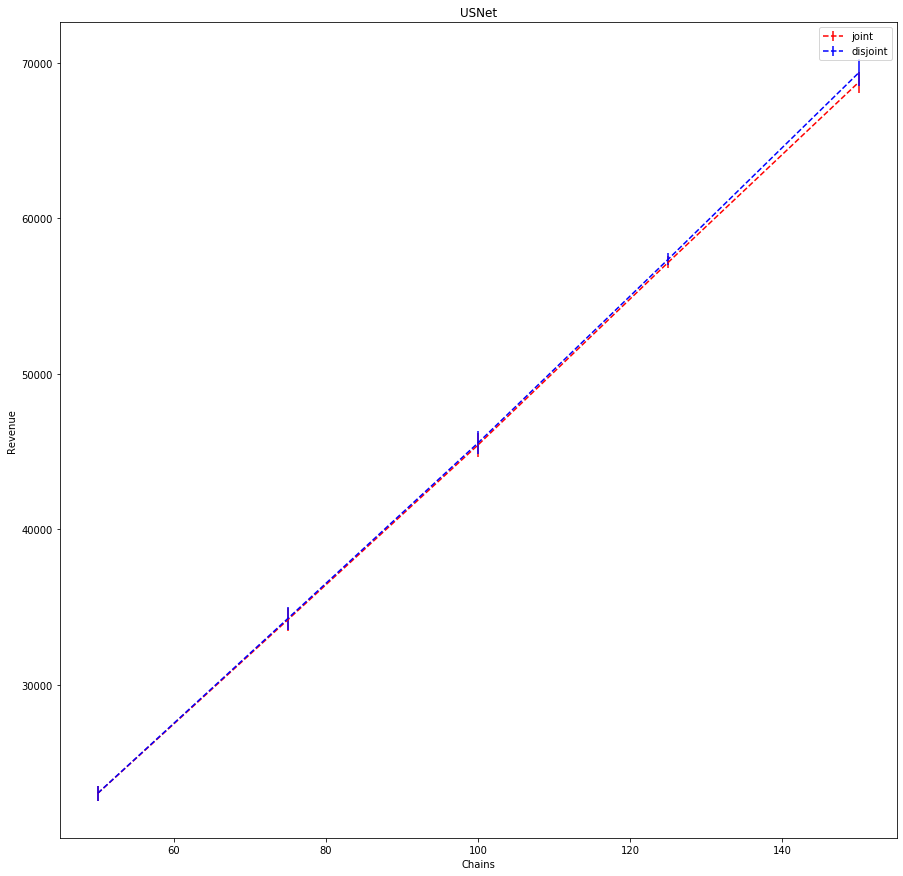
\includegraphics[height=350pt]{plots/joint-vs-disjoint-usnet.png}
    \caption{Revenues from Joint and Disjoint Solutions on USNet Topology}
    \label{fig:joint-vs-disjoint-usnet}
\end{figure}


\section{Conclusion and Future Work}
\hly{
a) Review of what we have done \\
b) What is the future step \\
}

\bibliography{references}

\end{document}
